\namedsection{mBed}{Gupta}

\note{Go through all tables and add references where required}
\note{Add a plan?}

\subsection{Introduction} \todo{Remove Title?}

mBed is a platform which implements ARM 32-bit processors within micro-controllers which is primarily developed by ARM. They are of the DIP form factor with 40 pins. It features an online SDK allowing for the development of projects online. It permits code to be written online as well as compiled into a binary compatible with the board being used. This binary can then be downloaded removing the pre-requisite of having the ARM toolchain available locally. The manner of uploading to the mBed is relatively straight forward with the presence of the mBed interface. \cite{mbed_website}\todo{Try expanding on this section}

This interface exposes a Mass Storage device to the host computer via a USB connection allowing for binaries to be uploaded in a drag and drop manner. The interface is also connected with the target chip using a JTAG connection allowing for it to program its flash memory. When the reset button is pressed, the interface checks the storage for the newest binary file and, should it not be programmed within the device already, will program the binary provided into the flash memory of the chip. \cite{mbed_website}\todo{Try expanding this section as well}

\subsection{Why the mBed}
\note{Need a better name for this subsection?}

When initially looking at various ways to emulate the sub-threshold version of the ARM Cortex M0, using an existing non sub-threshold version of the ARM Cortex M0 was considered. This involved searching for some form of micro-controller or device which would allow for programming of the processor. This lead to the mBed family which appeared easy to program and use featuring ARM processors. Within the mBed family of micro-controllers, the LPC11U24 model uses an ARM Cortex M0 as its processor.

An important factor for the device is being able to communicate with other devices using various communication protocols. Fortunately, multiple pins are broken out on the mBed which allow for flexibility in choice, in particular there are 2 SPI, 1 I2C, and 1 Serial interfaces available simultaneously upon the mBed. \cite{mbed_website} 

For obtaining data from the sensor, it is most likely to use I2C or One-Wire communication, should it be I2C, the mBed would work well. It also allows for the Serial pins to be interfaced with the host PC allowing for debugging information to be transmitted to the host PC. 

The requirements for this project require the processor to be emulate the sub-threshold version which operates with a system clock in the range of a few hundred kHz to a few MHz. This would require a clock in the micro-controller which can operate at these frequencies and also be able to be set as the system clock.

The device typically runs at 48MHz using its Internal RC oscillator (IRC) as its system clock. However, it also has the ability to switch its system clock to be sourced from the internal Watchdog oscillator instead. 

This oscillator consists of two parts, an oscillator function which generates an analog clock (\verb|Fclkana|) as well as a divisor (\verb|DIVSEL|) which is used to divide the analog clock to the required output frequency (\verb|wdt_osc_clk|). The output frequency can be calculated using Equation~\ref{eq:wdt_osc_clk} and is within the range $ 9.4 $ kHz $ \leq \verb|wdt_osc_clk| \leq 2.3 $ MHz. \cite{mbed_datasheet}

\begin{equation}
	\label{eq:wdt_osc_clk}
	\verb|wdt_osc_clk| = \frac{Fclkana}{2 * (1 + DIVSEL)}
\end{equation}

Some concerns were made realising that the Watchdog oscillator has an error margin of $\pm 40\%$ for the frequency of Fclkana. In a meeting with the client, it was decided to carry forward with the device while paying attention to this margin and analysing the impact of it upon the project.

\subsection{I2C Communication}

\subsubsection{Sensor library}

The sensor used in this project, the MPU6050 within a Xadow board, has an online library available \cite{sensory_library}. It contains two separate classes, one called I2Cdev and the other MPU6050. 

The I2Cdev class contains an interface to the processors I2C class expanding its functionality and allowing for more abstract functions for the MPU6050 class. For example, functionality for reading or writing multiple bytes or words were implemented within this class.

The MPU6050 class contains the functionality for configuring the sensor itself as well as reading data that it collects. It uses the I2Cdev class for communicating with the sensor.

The libraries are written for use with the Atmel chipset which use different libraries than those used by the ARM chipset. This poses a small issue as this means that the I2Cdev class would be incompatible for the ARM chip in use. In turn, due to the reliance on this class by the MPU6050 class, it would also be incompatible. 

This can easily be rectified by re-writing the I2Cdev class to make it compatible with the ARM libraries, which would also make the MPU6050 compatible.

\subsection{Watchdog Oscillator}

As mentioned before, one of the objectives of this project is to operate at a low operating frequency. It has already been seen that the Watchdog oscillator can operate in the desired frequency range using an analog clock as well as a divisor. 

To configure the Watchdog oscillator, it needs to be configured, powered on and then switched to. To do this, there are four registers that need interaction with to complete. The first register is the Watchdog oscillator control register (\verb|WDTOSCCTRL|) which contains the \verb|DIVSEL| and \verb|FREQSEL| talked about earlier. 

The lowest five bits of the register contains the unsigned value of \verb|DIVSEL|, hence allowing it to be within the range $ 0 \leq $ \verb|DIVSEL| $ \leq 31$. Thus, allowing for the divisor being within the range $ 2 \leq $ divisor $ \leq 64$.

The next four bits contains a value for \verb|FREQSEL|, where a value within the register corresponds to a different frequency with the relationship that can be seen in Table~\ref{tab:freqsel}.

\begin{table}
	\centering
	\begin{tabular}{|c|r|}
		\hline
		Value & Frequency \\
		\hline
		0x1 & 0.6 MHz \\
		0x2 & 1.05 MHz \\
		0x3 & 1.4 MHz \\
		0x4 & 1.75 MHz \\
		0x5 & 2.1 MHz \\
		0x6 & 2.4 MHz \\
		0x7 & 2.7 MHz \\
		0x8 & 2.0 MHz \\
		0x9 & 3.25 MHz \\
		0xA & 3.5 MHz \\
		0xB & 3.75 MHz \\
		0xC & 4.0 MHz \\
		0xD & 4.2 MHz \\
		0xE & 4.4 MHz \\
		0xF & 4.6 MHz \\
		\hline
	\end{tabular}
	\caption{FREQSEL table for WDTOSCCTRL register}
	\label{tab:freqsel}
\end{table}

With the available frequency values and divisors, it confirms the range that the Watchdog oscillator achieves which was given earlier.

The next register is the Power configuration register (\verb|PDRUNCFG|), which controls the power distribution to various analog blocks. At reset, the Watchdog oscillator is not powered meaning that before switching the system clock to it, it requires to be powered on. The bit that controls this is the sixth bit within the register, and toggling that bit to a value of 0 powers up the Watchdog oscillator. 

The next register (\verb|MAINCLKSEL|) sets the system clock to the Watchdog oscillator from the default IRC oscillator. This is stored in the lowest two bits of the register and potential values can be seen in Table~\ref{tab:sysclocksource}. As can be seen, for the system clock to use the Watchdog oscillator, the bottom two bits of the register need to be 0x2.

\begin{table}
	\centering
	\begin{tabular}{|c|l|}
		\hline
		Value & Source \\
		\hline
		0x0 & IRC Oscillator \\
		0x1 & PLL input \\
		0x2 & Watchdog Oscillator \\
		0x3 & PLL output \\
		\hline
	\end{tabular}
	\caption{Sources for the system clock}
	\label{tab:sysclocksource}
\end{table}

However, this does not automatically switch the system clock to use the Watchdog oscillator. It is required for the system clock to be updated before any change takes place, this is done in the final register (\verb|MAINCLKUEN|) within its least significant bit. For the update to take place, the value in this bit needs to change from a 0 to a 1. The reset value within this bit is 1, and thus it is required for it to first be set as 0 before switching it to 1.

After all the register changes have taken effect, the system clock is configured to source itself from the Watchdog oscillator allowing the mBed to operate in the correct frequency range to simulate the sub threshold processor.

\subsubsection{Analysing the error margin}

It is known that the Watchdog oscillator has an error margin of $ \pm 40\%$, the actual impact this would have however is unknown. According to the data sheet \cite{mbed_not_datasheet}, the primary reason for this is temperature. Due to the conditions that the device is intended for, upon a plane, the ambient temperature can be assumed to not be at extreme temperatures in either direction, hence should not be an issue. There was a hypothesis that the power supply voltage could also affect the frequency of the oscillator. 

To test this, the supply voltage for the mBed is varied and the output frequency of the oscillator is checked. There was an issue due to the fact that the mBed does not provide a breakout pin for the CLKOUT pin. To get around this, the while loop is programmed to contain only toggling a pin. The act of toggling the pin should take a constant number of cycles each time, hence the frequency of that pin should be proportional to the frequency of the clock. Hence, can be used to measure deviations in the system clock.

Implementing this with the watchdog oscillator using a FCLKANA of 0x1 (0.6 MHz) and a DIVSEL of 2 (Divisor of 6), the Watchdog oscillator oscillates at 100 kHz. Measuring the frequency of the pin over a range of voltages shows no change in frequency, hence disproving the hypothesis that the voltage would also affect the operating frequency.

\subsection{Serial Communication}

For the purposes of debugging, serial communication was used to extract information from the device and onto the host computer. To accomplish this, a C232HM cable \cite{c232hm_datasheet} was used to interface with the host computer, via USB, and the mBed, via Serial pins 9 and 10. The baud rate was left at the default value of 9600 and to test the communication, the mBed was programmed to send "Hello World!" to the host pc via Serial communication.

This communication was done when the device was operating at its default frequency of 48 Mhz where the libraries have the correct default values set in the registers to enable the correct divisors to enable the device to operate at 9600 baud. However, these would not be viable values when using the Watchdog Oscillator as the system clock.

\subsubsection{Serial Divisor}

To enable the device to communicate with the desired baud rate when the system clock is set at a lower frequency, the divisor needs to be configured. There are multiple registers that need to be modified to achieve this. The first two are the DLL and DLM registers. These registers, within the lowest eight bits, contain the DLL and DLM bytes respectively, where DLL is the least significant byte of the Divisor Latch (DL) and DLM is the most significant byte.

For access to be granted to the DL, the Divisor Latch Access Bit (DLAB) needs to be set. This value is stored within the Line Control Register as the seventh bit. The final register is the Fractional Divide Register which contains the DIVADDVAL and MULVAL values. DIVADDVAL is stored within the lowest four bits, whilst MULVAL is stored within the next four lowest bits. 

Using these values, the baud rate can be calculated using Equation~\ref{eq:serial_baud_rate} where PCLK is the clock frequency\cite{mbed_datasheet}.

\begin{equation}
	\label{eq:serial_baud_rate}
	UART_{baud rate} = \frac{PCLK}{16 * (256 * DLM + DLL) * (1 + \frac{DivAddVal}{MulVal})}
\end{equation}

Within the mBed datasheet \cite{mbed_datasheet}, a methodology for calculating these values is provided which can be seen in Figure~\ref{fig:serial_algo}. Along with the algorithm, a look up table is provided which can be used to translate a FR value to DIVADDVAL and MULVAL values. 

\begin{figure}
	\centering
	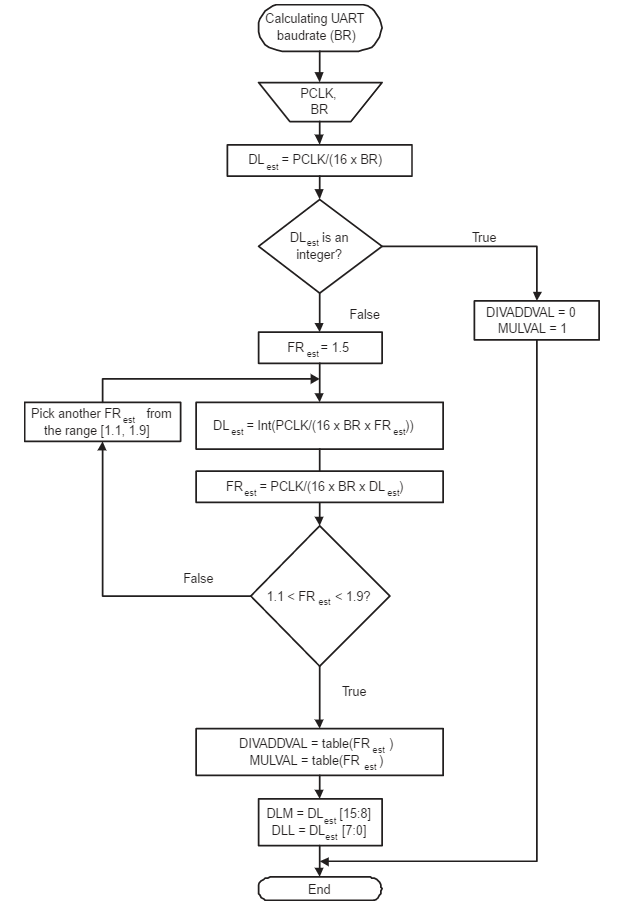
\includegraphics[scale=.85]{usart_algorithm.png}
	\caption{Algorithm to calculate required values for Serial baud rate}
	\label{fig:serial_algo}
\end{figure}

\subsubsection{Auto-Baud}

Another option to account for this is a feature provided within the processor called Auto-Baud\cite{mbed_datasheet}. This is where the device waits on receiving communication upon its RX pin and of the data coming in, it measures the baud rate between a falling edge and a subsequent rising or falling edge depending on the mode set within the registers.

Using this information, the required registers are set to enable Serial communication such that the device can communicate at the required baud rate. To enable an effective method for enabling auto baud, a python script was created which can be used on the host PC. This script continuously sends the character 'g' whilst also receiving and printing bytes. The continuous stream of 'g's gives a signal for auto baud to configure itself and should the device be reset during communication it will be configured automatically after reset should the script be running.

\subsection{Getting Sensor Data}

\note{Should this be moved to the I2C subsection?}

With the sensor libraries re-written to be compatible with the ARM libraries, the sensor can be interfaced with the mBed. Upon the sensor, all pins used were on Junction 4. This pins connected between the mBed and sensor were the data line, pins 28 and 3 respectively, as well as the clock line, pins 27 and 2 respectively. These pins were also connected to pull-up resistors with values of 2.2k\ohm. Power was also supplied to the sensor from the mBed from its 3.3V Regulated Output which went to pin 1 of the sensor along with a common ground between the Ground pin of the mBed and pin 6 of the sensor. 

Once done, it was possible to extract sensor readings from the device, depending on what data is required a variety of different functions from the library can be used.

\begin{description}
	\item[Accelerometer X axis] \hfill \\ getAccelerationX
	\item[Accelorometer Y axis] \hfill \\ getAccelerationY
	\item[Accelorometer Z axis] \hfill \\ getAccelerationZ
	\item[Accelerometer all axis] \hfill \\ getAcceleration
	\item[Gyroscope X axis] \hfill \\ getRotationX
	\item[Gyroscope Y axis] \hfill \\ getRotationY
	\item[Gyroscope Z axis] \hfill \\ getRotationZ
	\item[Gyroscope all axis] \hfill \\ getRotation
	\item[Accelerometer and Gryoscope all axis] \hfill \\ getMotion6
\end{description}

\todo{Do something about this}

Thus allowing for a variety of possibilities for obtaining data from the sensor, as should only certain data be required, a function can be chosen which reduces the amount of data being received, hence reducing the communication time between the mBed and sensor.

\subsection{Getting the desired sampling rate}

The model employed requires a set sampling rate, and to minimise the communication between the mBed and device to minimise processing, the mBed should sample the sensor at the sampling rate required by the model. To achieve this, there a few different parameters tweaked, specifically the Watchdog \verb|FCLKANA| and \verb|DIVSEL| as well as SCLL and SCLH for the I2C clock. These values represent the number of clock cycles the I2C clock remain low and high respectively, where the lowest value they may have is four. Thus, can be used to speed up or slow down I2C communication. \cite{mbed_datasheet} This can be summed in Equation~\ref{eqn:i2c_clock}.

\begin{equation}
	I2C_{clock} = \frac{CLK}{SCLH + SCLL}
	\label{eqn:i2c_clock}
\end{equation}

It was decided that the duty cycle of the I2C clock is 50\%, hence the value of SCLL and SCLH should be the same. A similar method, from when measuring the frequency of the oscillator with varying voltage via a pin, was used where the frequency of the pin is half the sampling rate. This because in one cycle of the pin, it goes through the while loop twice and the sensor is queried once each loop.

\subsection{Issues}

There were a variety of issues that were encountered with the mBed. It was possible to remedy some of the issues, however not all.

It was found that forgetting to power on the Watchdog oscillator before switching the system clock over to it left it in a state where it was unable to execute any code. This state, for unknown reasons, persisted even after a reset and reboot of the device. An eventual solution to this problem was found, which was to re-flash the mBed interface firmware.

SPI communication was attempted to interface the mBed to a SD card allowing for data from the sensor to be stored within the SD card so it is possible to revisit collected data at a later point in time. This would be especially useful should the device not be connected to the host PC to send debug information to. Navigating the mBed site does show a library with functionality perfect for this aim, however attempting to compile the example code resulted in a error during compilation due to the fact the binary would have been larger than the flash capacity of the mBed. Switching over to the online compiler provided by mBed resulted in compilation however the binary would not execute upon the mBed.

An issue occurred when optimising multiple multiplication and division operations into a single bit shift however, the output of said optimisation caused the code to return different results compared against the unoptimised version upon the mBed however not on another machine. This was found to be due to the fact that the mBed stores its variables in a little endian format.

\subsection{Measuring power}

It is required to measure the power of the system as a requirement is for it to be low powered as the sub threshold processor will be operating at a low power. It was deemed unnecessary to measure the power consumption of the mBed because of the various peripherals which are also powered which would not be there on the sub threshold version as well as the fact that this processor is not designed for sub threshold power and the method ARM implement to achieve this may leave a different power fingerprint than the Cortex M0. 

The sensor however does not fall under the same conditions and thus, was analysed for its power usage. To do this a 100\ohm ~resistor was placed in series between the sensor and $V_{cc}$. Thus current would have to flow through the resistor to reach the sensor, allowing to measure the current by measuring the voltage across the resistor along with the relationship V=IR.

The power consumption of the sensor is not constant over time due to the fact that the sensor alternates between sleep mode and being awake. It also will consume more power when communicating over I2C as opposed to not. To account for this, the current and voltage is measured over time which is then averaged thus, giving the average power consumed by the sensor.

\begin{table}
	\centering
	\begin{tabular}{|l|r|r|}
		\hline
		Parameter & Mean Value & Standard Deviation \\
		\hline
		Resistor Voltage (V) & 0.0262 & 0.00198 \\
		Sensor Voltage (V) & 3.29 & 0.00133 \\
		Current (A) & 0.000262 & \\
		Power (W) & 0.00086198 & \\
		\hline
	\end{tabular}
	\caption{Power statistics for the sensor}
	\label{tab:power}
\end{table}

As can be seen from Table~\ref{tab:power}, the sensor on average took $861\mu W$ which can be considered low power. However, there is the potential for a lower power consumption, within the configuration used, the current flowing through the sensor was $262\mu A$, but the data sheet for the sensor says for the sampling rate and configuration that is being used, the typical value is $70\mu A$. This decrease would reduce the power consumption by over a factor of 3 leaving a power usage of $230\mu W$.

\subsection{Prototyping}

During development, breadboard was used to prototype the system with both the mBed and sensor placed upon. The power rails on the breadboard received power from the mBed which in turn received power from the host PC via USB. These conditions were acceptable when developing, however was impractical for moving the device to the foot for further testing. 

It was decided to create a small board for this purpose using veroboard which would be powered with a few AA batteries. This is beneficial as the board can be made to a desired size with on-board power alleviating the requirement of having a cable trailing to a computer as well as being more comfortable on the foot over the breadboard.

A design was created using fritzing \cite{fritzing} which can be seen in Figure~\ref{fig:veroboard_schematic}. The mBed has a $V_{in}$ pin upon pin 2 which can take from 4.5V up to 9V which is supplied using four AA batteries within two AA battery holders. To prevent the mBed from constantly being powered, a jumper is added to control whether the mBed receives power or not enabling for the device to be switched on or off at will. Power to the sensor is provided via the 3.3V regulated output of the mBed, which also is used by the pull-up resistors to hold the I2C lines high when not in use. Extra space was added above and below the sensor due to the fact that the physical board is larger than that in the CAD software upon that axis, thus requires more space to avoid colliding with the mBed or hanging off the edge of board.

\begin{figure}
	\centering
	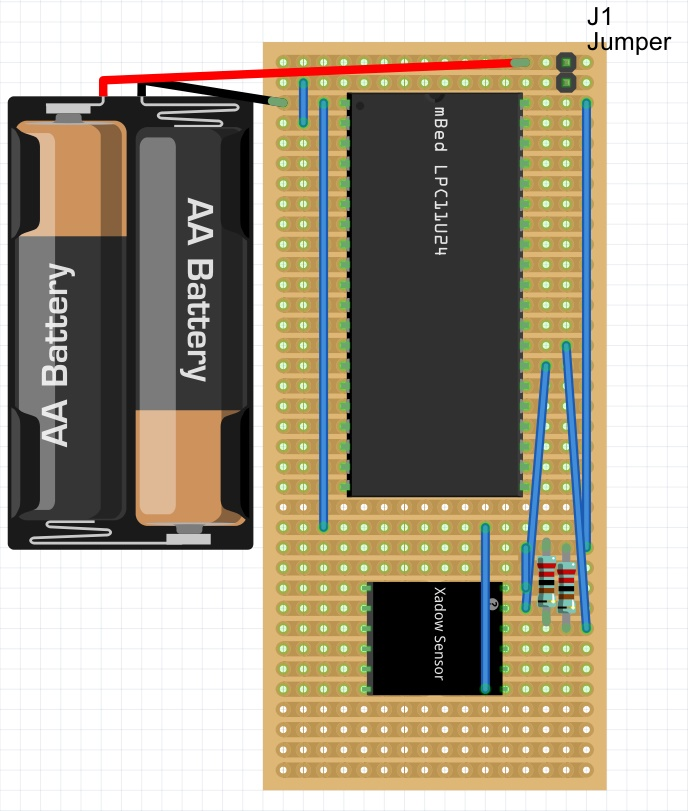
\includegraphics[scale=.6]{veroboard_schematic.png}
	\caption{Schematic for veroboard}
	\label{fig:veroboard_schematic}
\end{figure}

This was then built, as can be seen from Figure~\ref{fig:board}. To avoid having to solder on the actual mBed and sensor to the veroboard, female header pins are used in a manner similar to IC holders allowing for them to be placed and removed from the board as required. For compactness, the battery packs were attached to the underside of the board using velcro. 

\begin{figure}
	\centering
	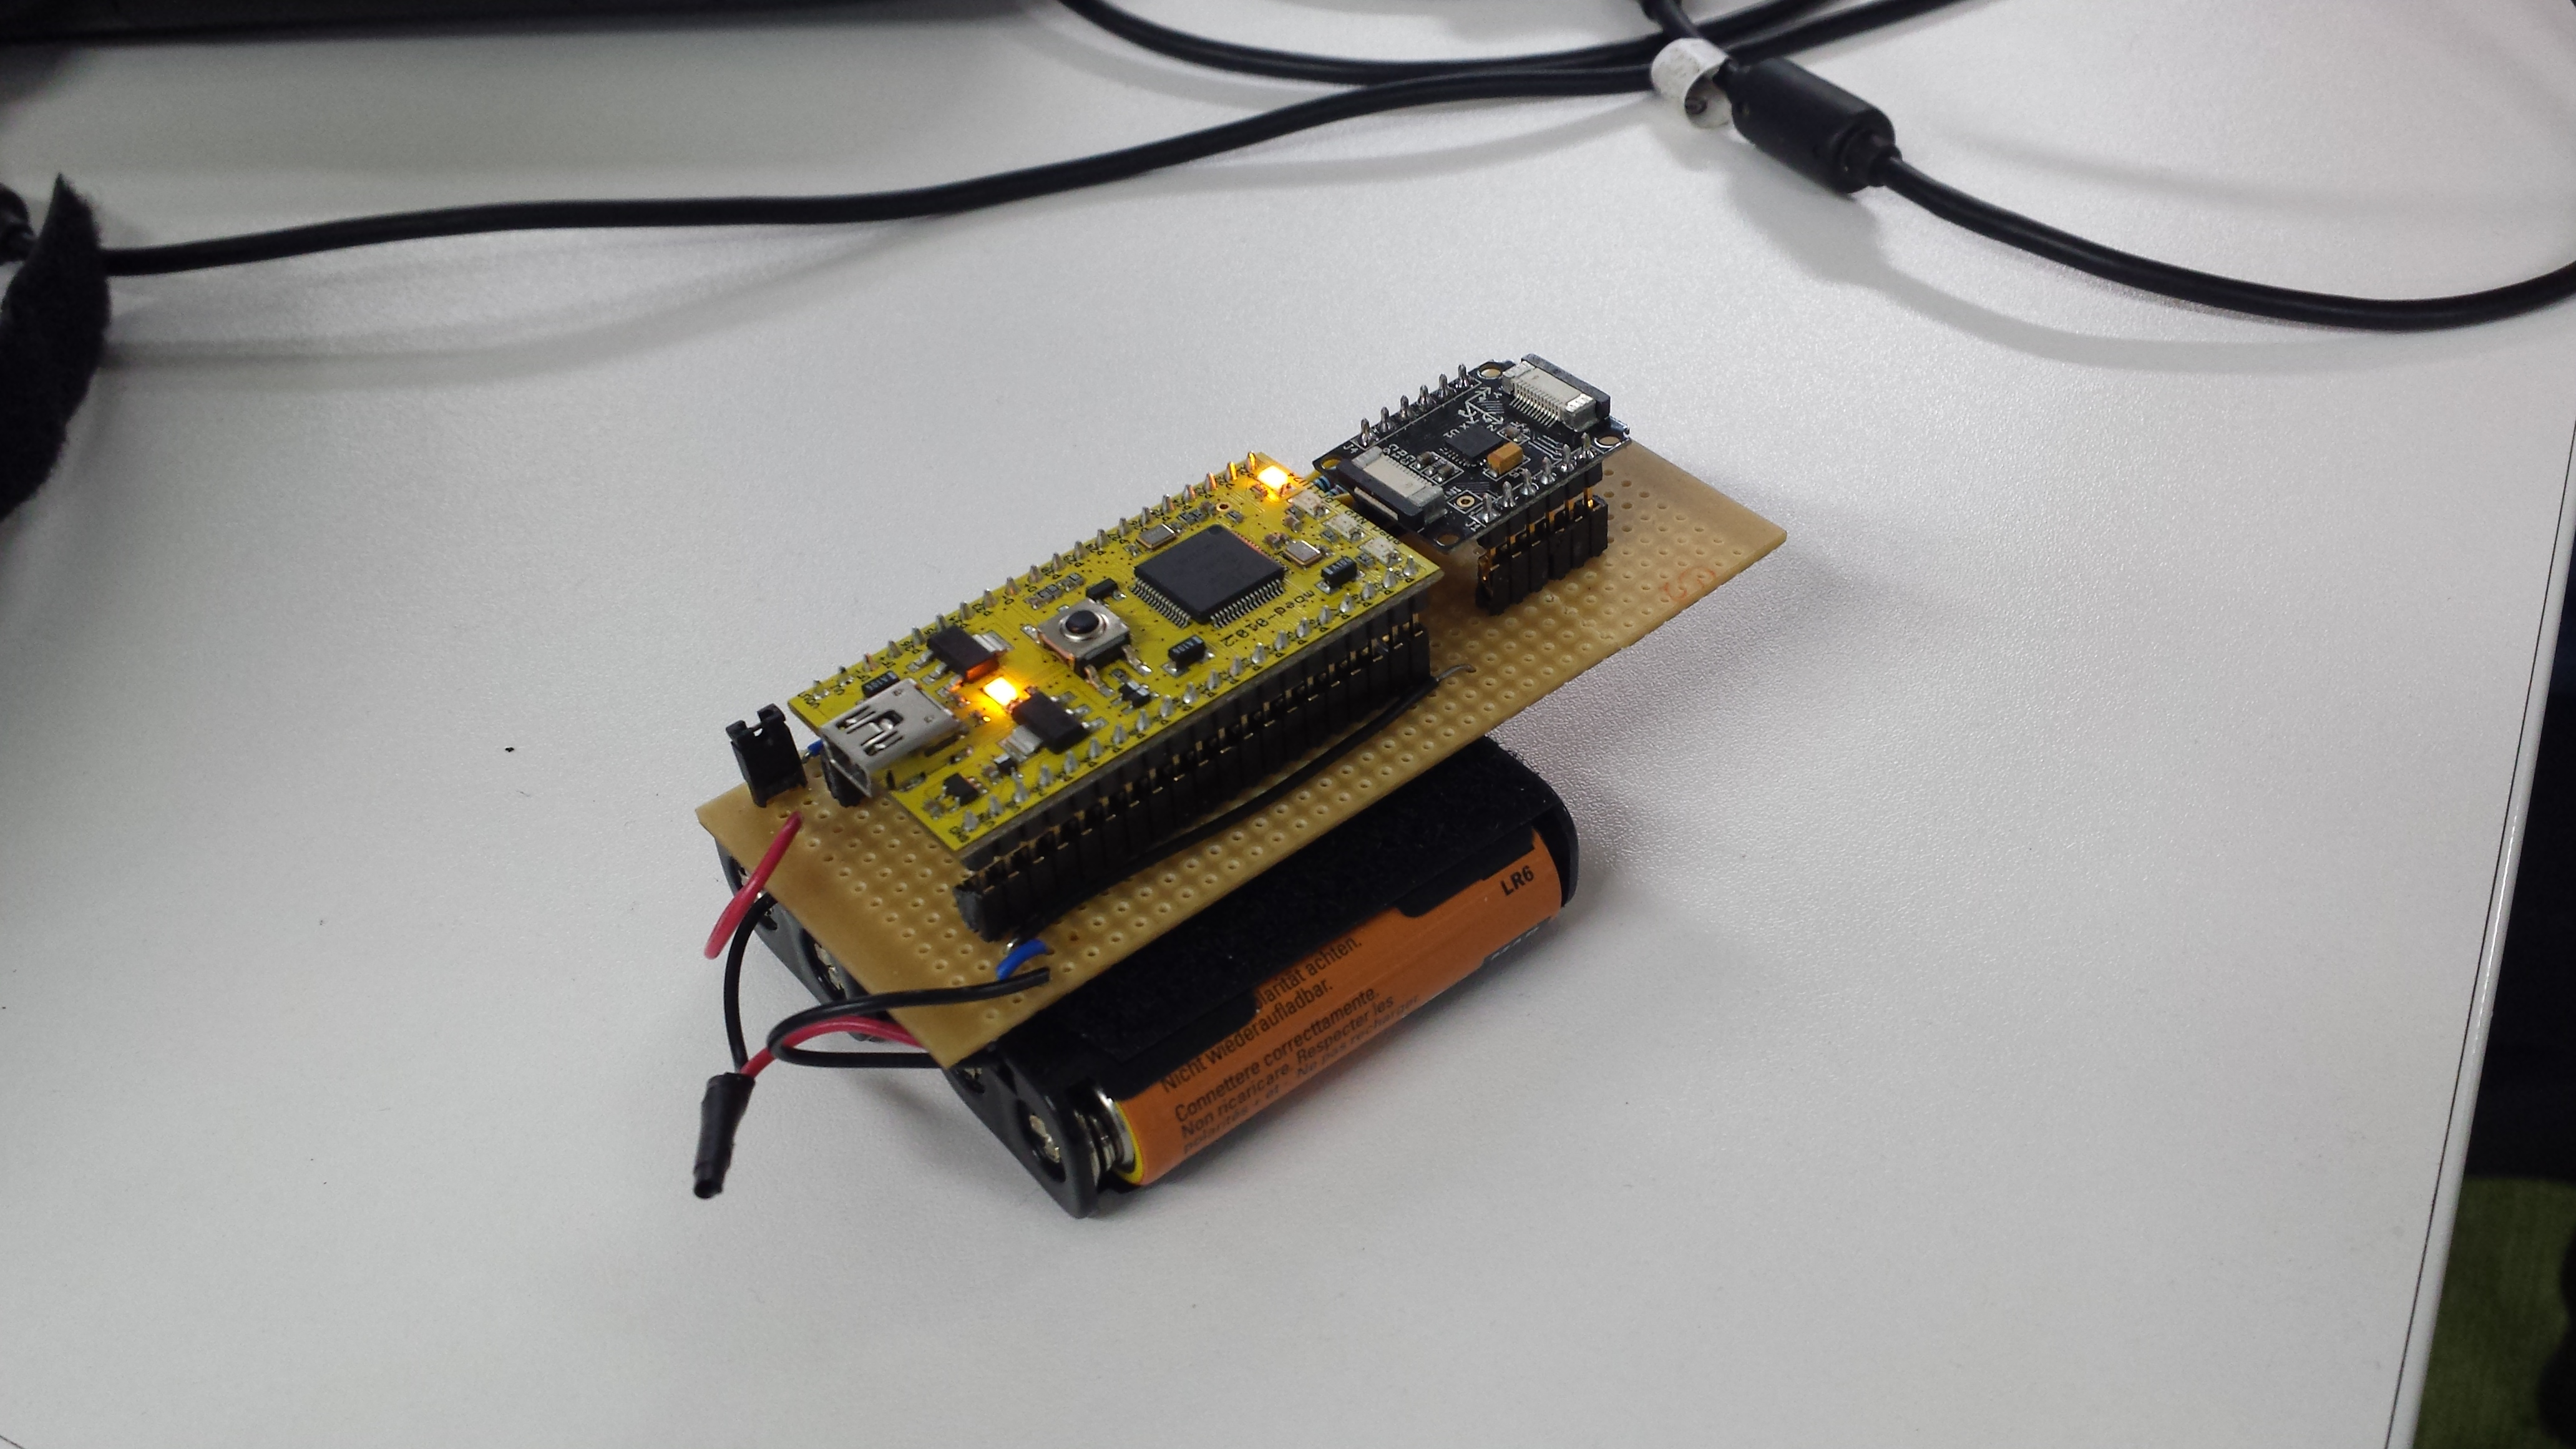
\includegraphics[scale=.1]{prototype_no_straps.jpg}
	\caption{Prototype board}
	\label{fig:board}
\end{figure}

The board was now able to be placed upon a foot, however there was nothing to secure it in place. A similar approach was taken from the participant study of using velcro. Two pieces of velcro would be attached to the board, whilst another two to the foot. This would then allow the board to be placed on the foot with the velcro holding the board onto the foot. The reasoning for using two pieces of velcro over one is that it was found to allow for more stability when on the foot over one piece where it leaves room for the board to start rotating forwards and backwards. The board with the velcro can be seen in Figure~\ref{fig:board:velcro}.

\begin{figure}
	\centering
	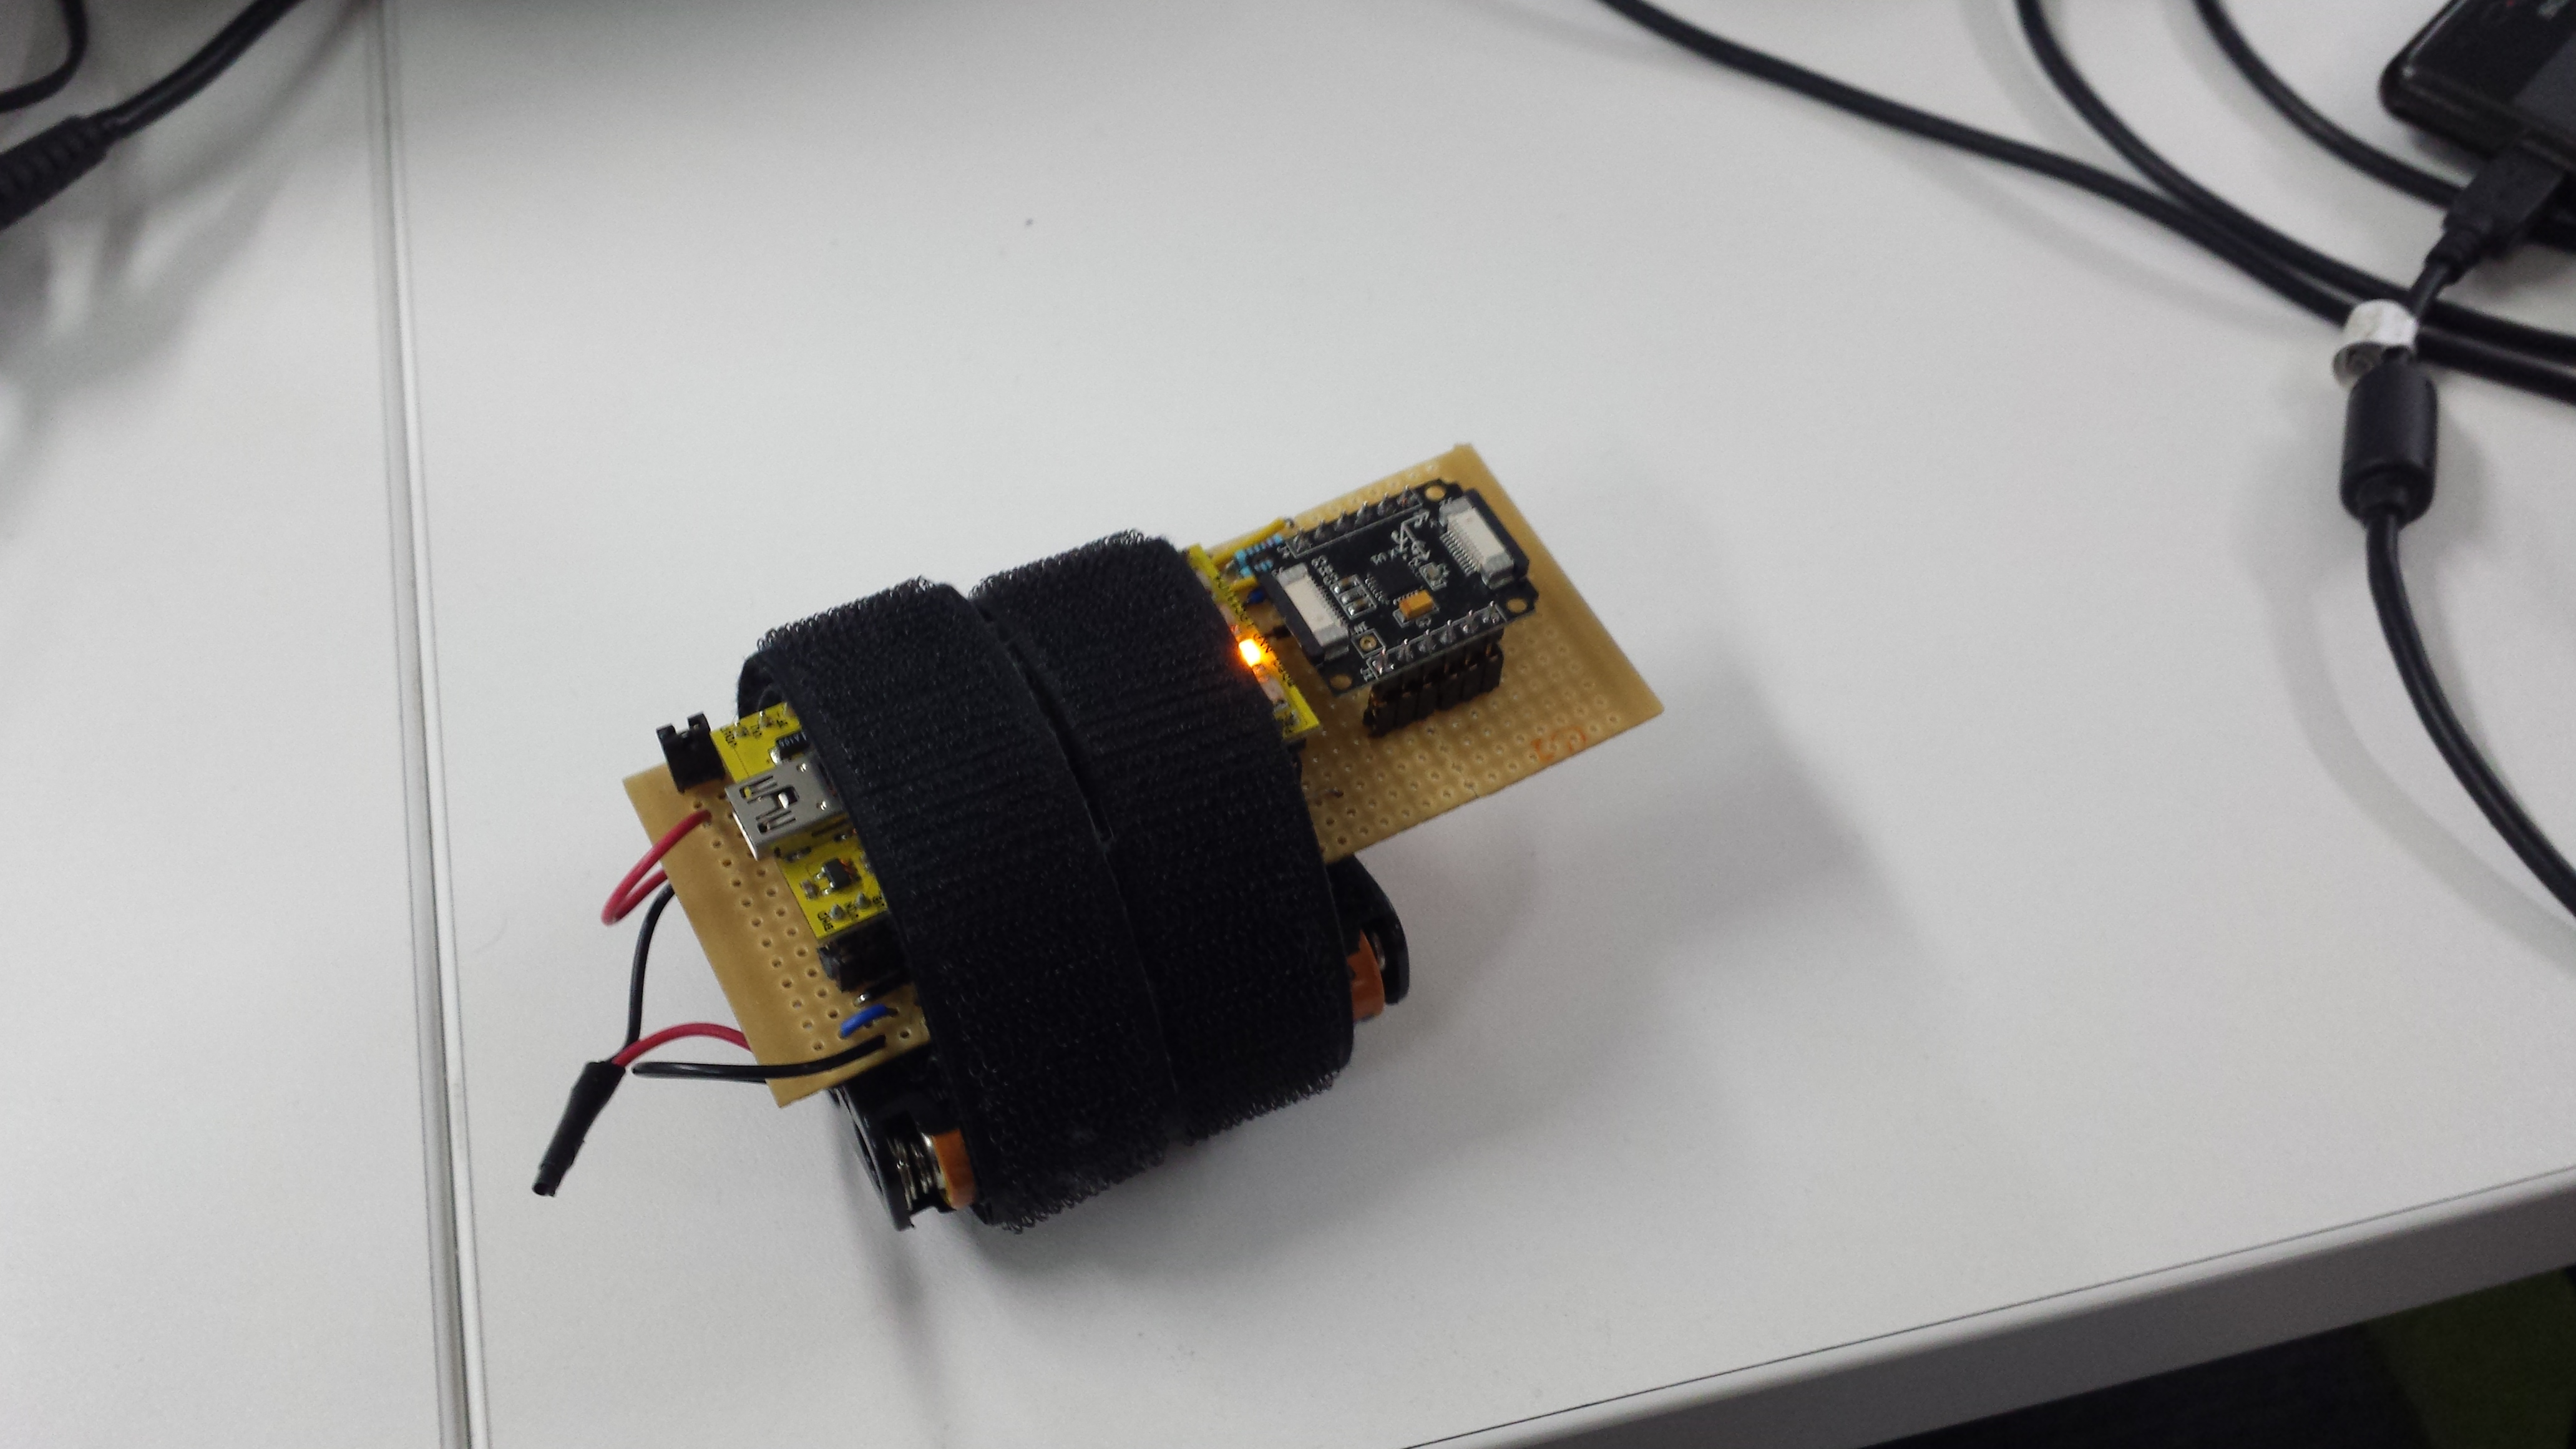
\includegraphics[scale=.1]{prototype_straps.jpg}
	\caption{Prototype board with velcro straps}
	\label{fig:board:velcro}
\end{figure}